

\chapter{User Interface Design}
\section{General Overview}
The User Interface of \textbf{Best Bike Paths} follows a strict \textbf{map-centric approach}, optimized for outdoor usage to ensure high legibility and safe, single-handed interaction while cycling. 

\noindent
The navigation is anchored by a persistent Bottom Navigation Bar, allowing rapid access to core features, while the layout dynamically adapts content based on the User's authentication state. To minimize cognitive load during physical activity, the design adheres to three key principles:
\begin{itemize}[noitemsep]
    \item \textbf{Usability and Safety:} High-contrast color schemes and enlarged touch targets are used to facilitate interaction under varying lighting conditions and movement.
    \item \textbf{Data Hierarchy:} The interface clearly separates dynamic performance metrics (Trips) from static geographical data (Paths).
    \item \textbf{Transparency:} Mandatory safety disclaimers are presented upon startup to set clear User expectations.
\end{itemize}


\section{User Interface Layouts}
\subsection{Landing Screen}
\begin{figure}[H]
    \centering
    \begin{subfigure}[b]{0.23\textwidth}
        \centering
        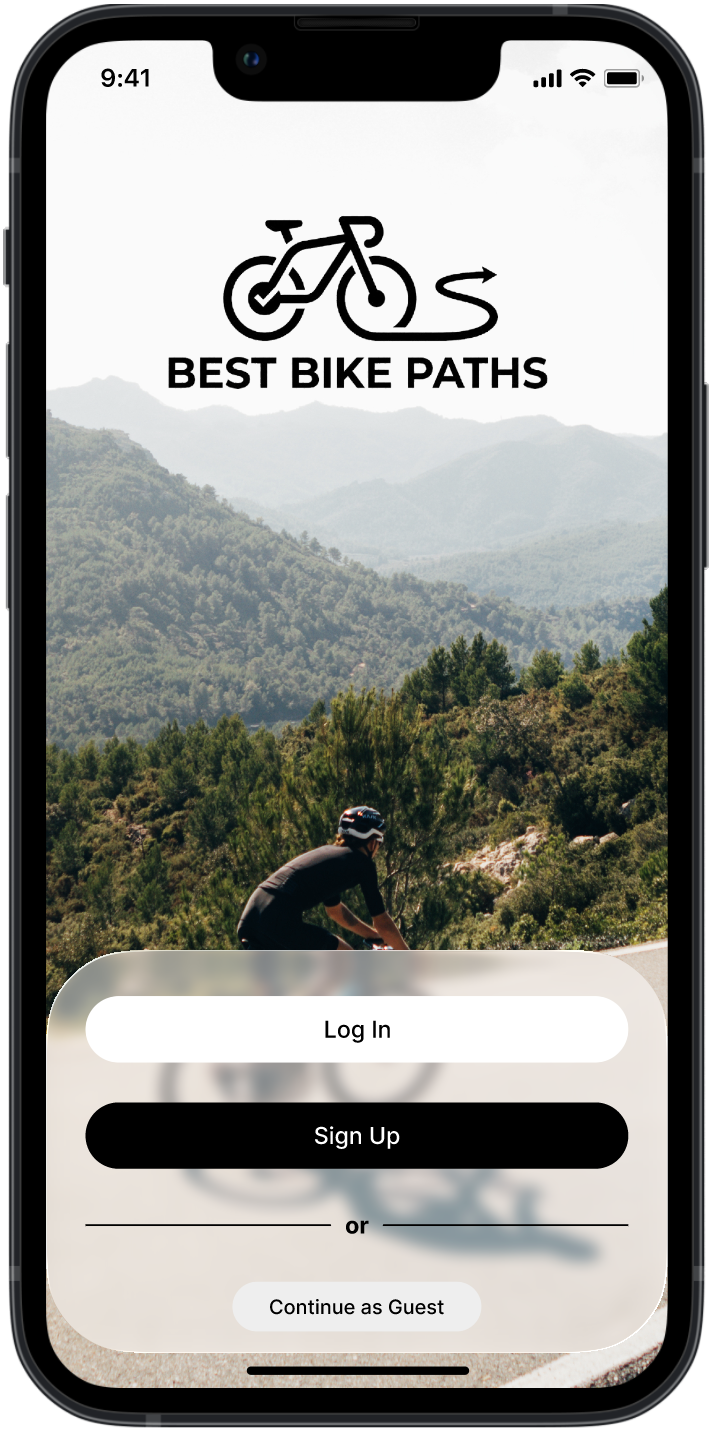
\includegraphics[width=\linewidth]{figures/mockup/landing_screen.png}
        \label{fig:landing_screen}
    \end{subfigure}
    \hfill 
    \begin{subfigure}[b]{0.23\textwidth}
        \centering
        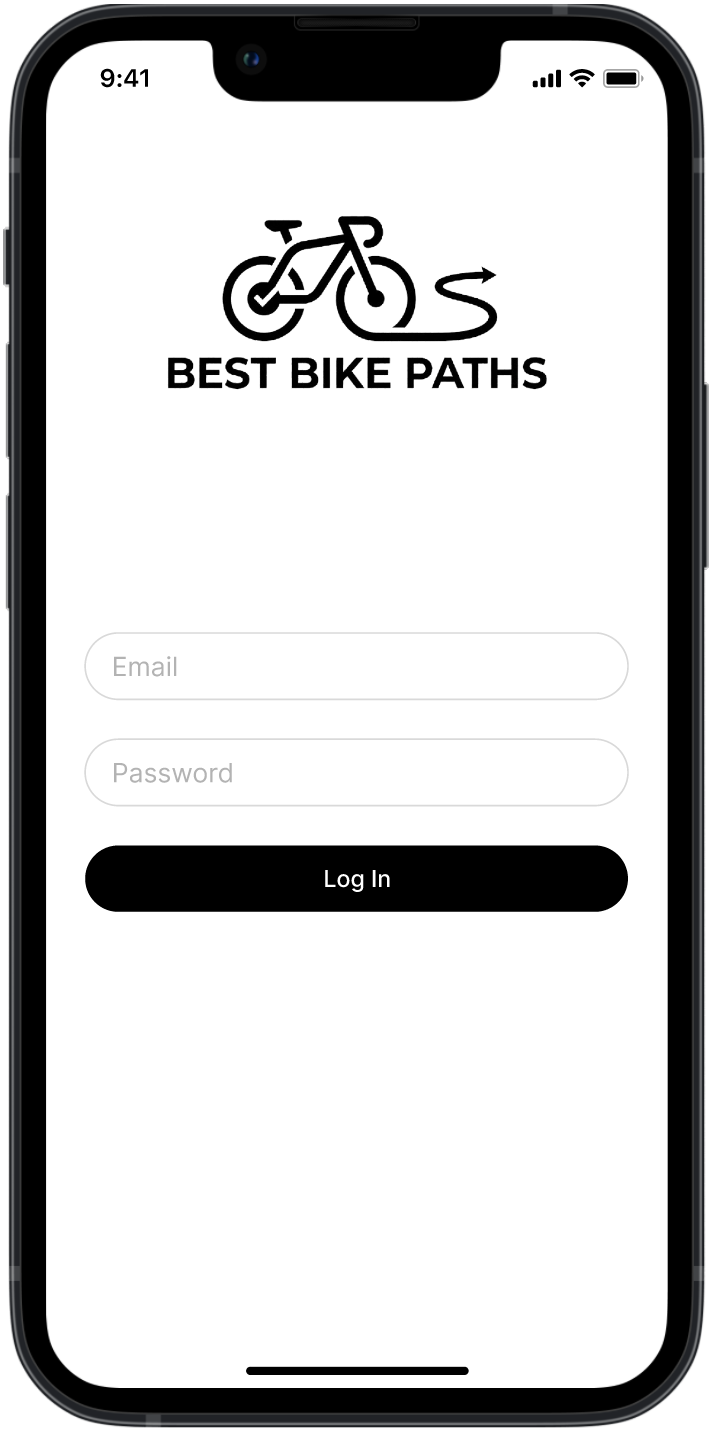
\includegraphics[width=\linewidth]{figures/mockup/log_in.png}
        \label{fig:log_in}
    \end{subfigure}
    \hfill
    \begin{subfigure}[b]{0.23\textwidth}
        \centering
        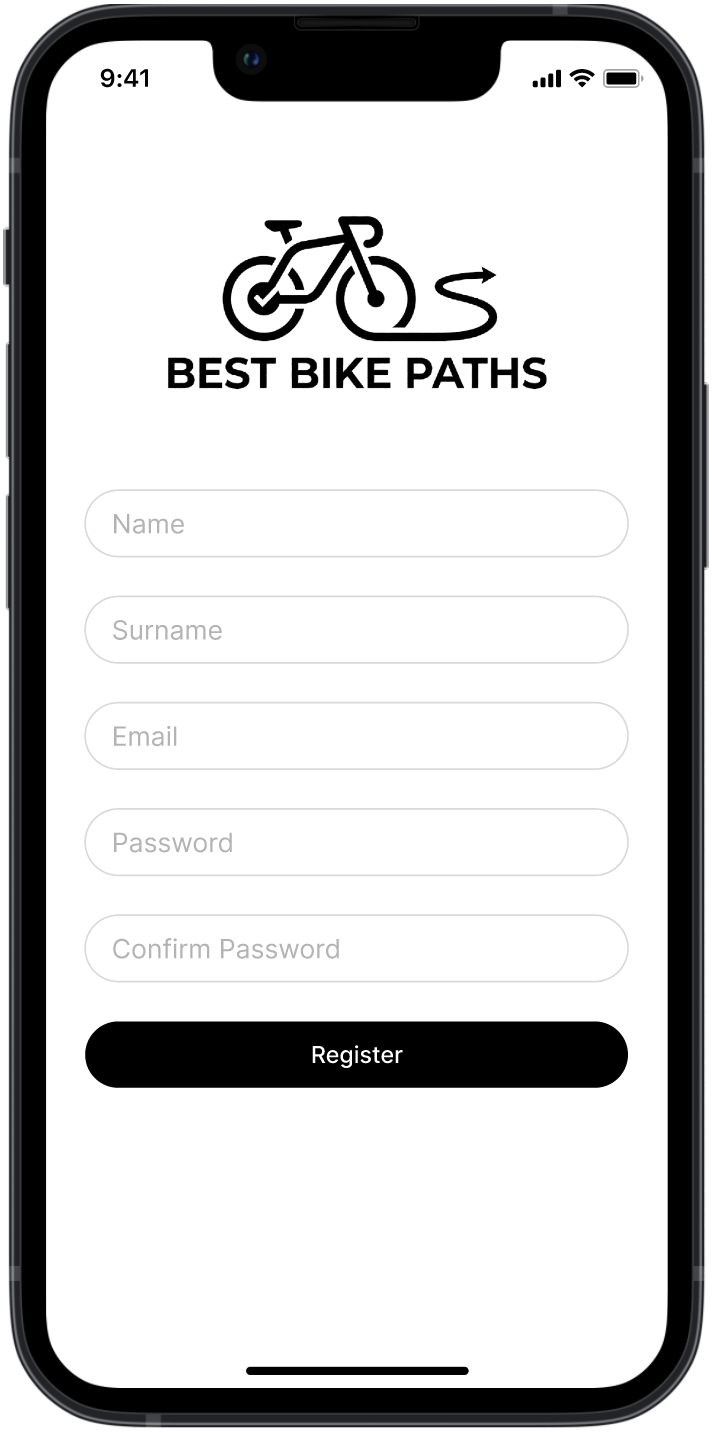
\includegraphics[width=\linewidth]{figures/mockup/sign_up.png}
        \label{fig:sign_up}
    \end{subfigure}
    \hfill
    \begin{subfigure}[b]{0.23\textwidth}
        \centering
        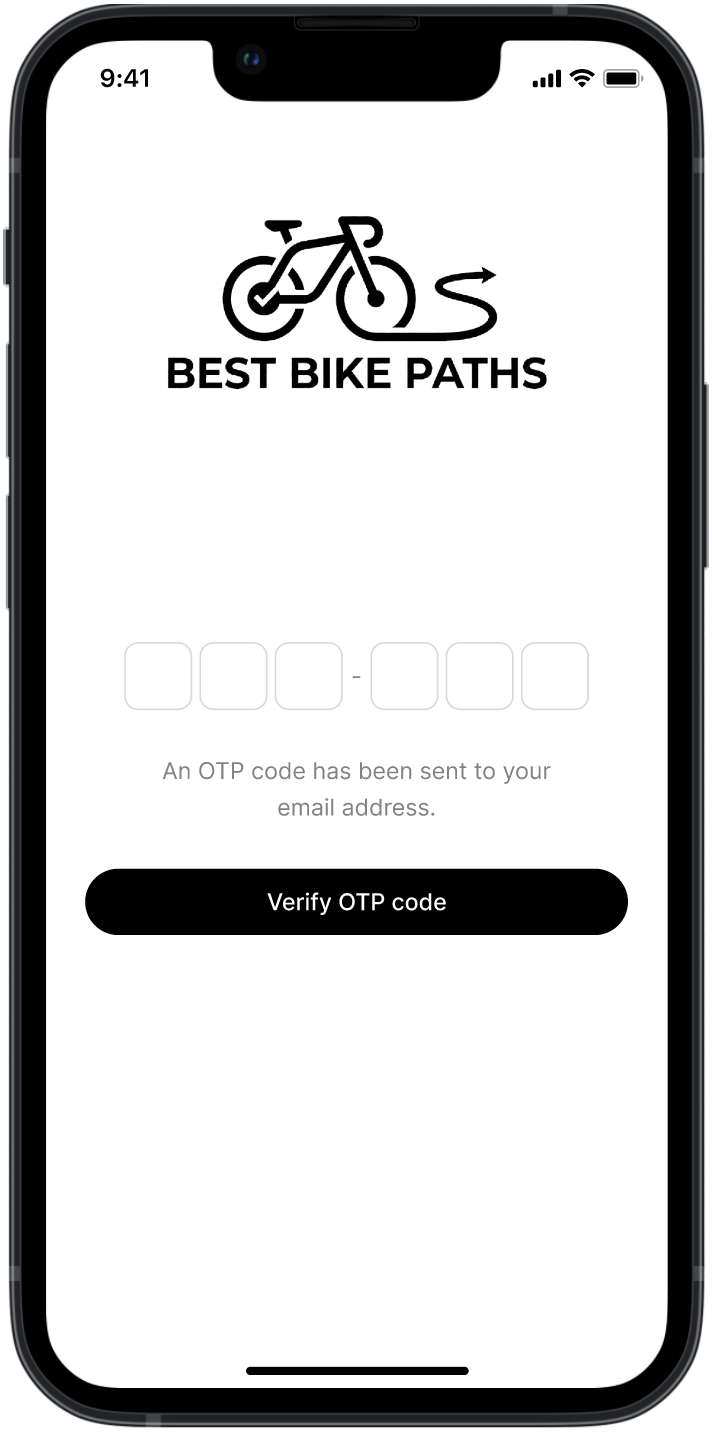
\includegraphics[width=\linewidth]{figures/mockup/verification_otp.png}
        \label{fig:verification_otp}
    \end{subfigure}
    
    \caption{Landing, Sign Up, and Sign In Screens}
    \label{fig:landing_screen}
\end{figure}

\vspace{-0.5cm}
The Landing Screen serves as the application's entry point and primary security gate. Its main purpose is to direct the User toward the appropriate operational mode based on their authentication status, ensuring that access privileges are enforced immediately upon startup.

The interface prioritizes User acquisition by presenting \textbf{Sign Up} as the primary call-to-action. This option is designed for new Users who intend to utilize the active features of the application, such as recording Trips, earning statistics, and contributing data to the community. For returning Users who already possess valid credentials, the \textbf{Log In} functionality provides access to the authentication process, allowing them to retrieve their personal profile and historical activity data. Additionally, the screen provides a \textbf{Guest Access} entry point for unregistered Users, such as tourists or casual explorers. 

\subsection{Explore}
\begin{minipage}[t]{0.45\textwidth}
    \setlength{\parindent}{7mm}
    \setlength{\parskip}{2mm}
    \vspace{0pt}
    \noindent
    The Explore Screen acts as the primary navigational interface for the application. This section is accessible to all User categories, including unauthenticated guests. The interface is dominated by the \textbf{Interactive Map}, which shows the User location and their surroundings.
    
    The interface features a prominent \textbf{Start Recording} button, typically positioned as a Floating Action Button to ensure easy accessibility. The System implements a role-based behaviour for this control: for \textbf{Registered Users}, tapping the button immediately initiates the active recording flow. Conversely, for \textbf{Guest Users}, the interaction triggers a modal window informing them that performance tracking is a feature reserved for members, thereby prompting them to sign up to unlock the full potential of the application. This also happens when Guest Users try to navigate to the \emph{My Activity} section.
\end{minipage}
\hfill
\begin{minipage}[t]{0.50\textwidth}
    \vspace{0pt}
    \captionsetup{type=figure}
    \begin{subfigure}{0.48\linewidth}
        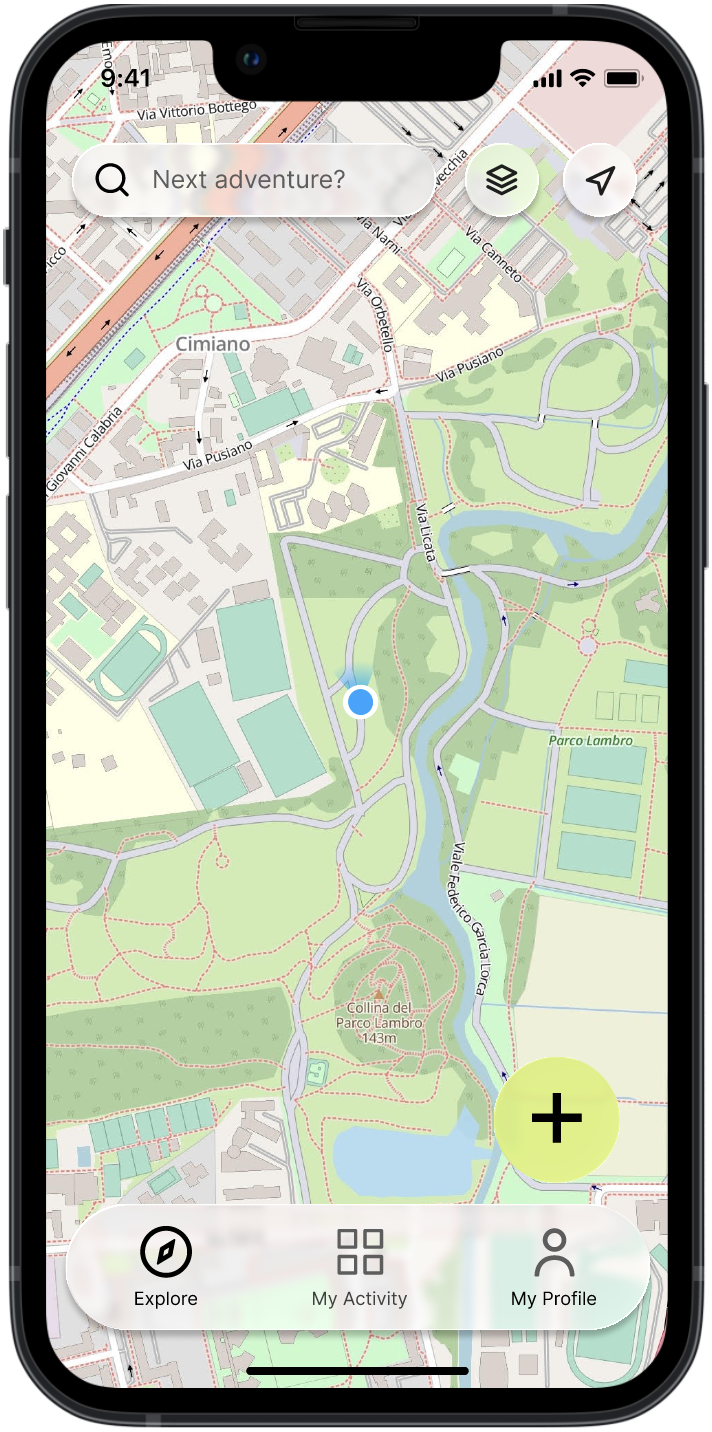
\includegraphics[width=\linewidth]{figures/mockup/explore_landing.png}
        \caption{Explore Section}
        \label{fig:explore_landing.png}
    \end{subfigure}
    \hfill
    \begin{subfigure}{0.48\linewidth}
        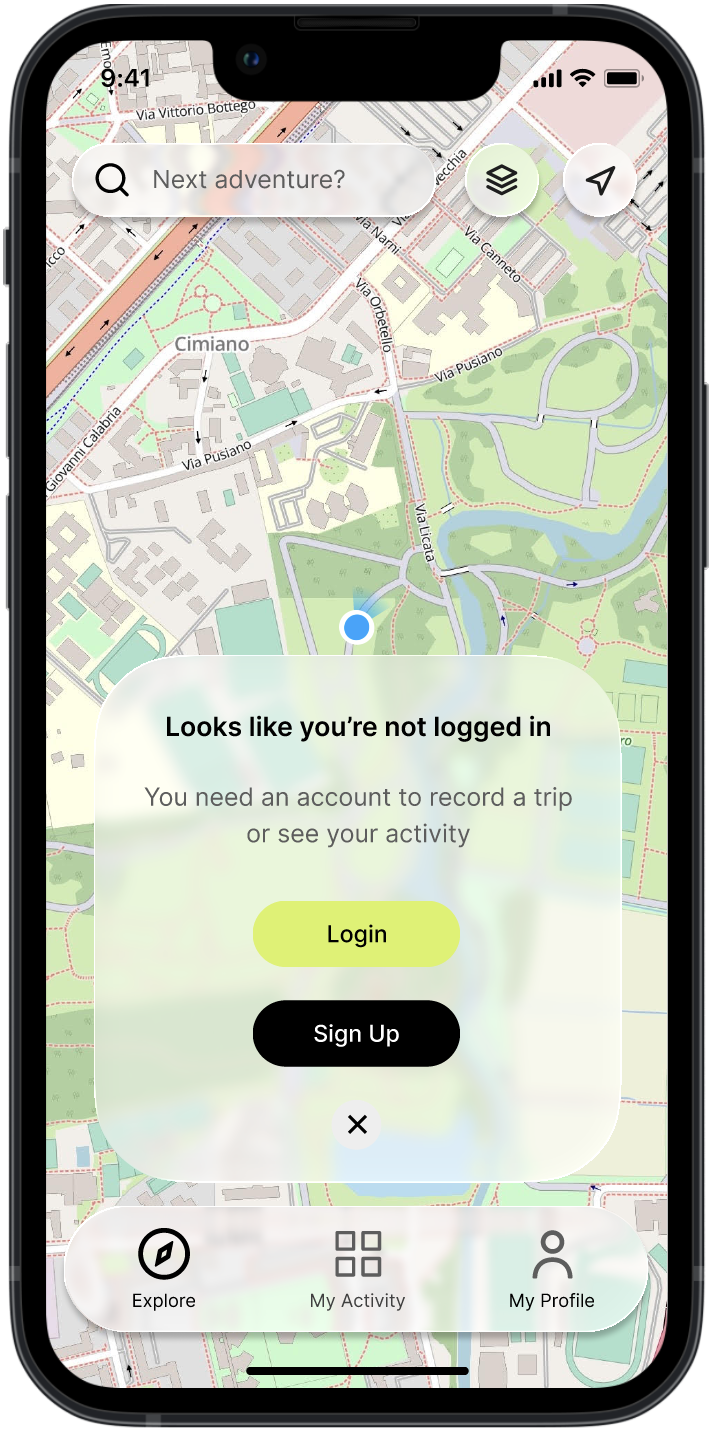
\includegraphics[width=\linewidth]{figures/mockup/explore_unregistered.png}
        \caption{Guest User modal window}
        \label{fig:explore_unregistered}
    \end{subfigure}
    \caption{Explore Section Screens}
\end{minipage}


\subsubsection*{Search}
\begin{minipage}[t]{0.45\textwidth}
    \setlength{\parindent}{7mm}
    \setlength{\parskip}{2mm}
    \vspace{0pt}
    \noindent
    The search workflow is managed through dedicated interfaces designed to guide the User from route definition to selection.
    
    The \textbf{Path Search Input} screen allows Users to define the route's starting point and destination. To streamline the interaction, the interface supports address auto-completion and direct point selection on the map.
    
    Upon submission, the System transitions to the \textbf{Search Results} screen, which presents the Pathfinding algorithm's output. The available routes are visualized on the map and listed as summary cards, ranked by their calculated \emph{Score}. Crucially, this view provides more than just distance and duration; each option highlights the aggregated \textbf{Path Status} and specific \textbf{Warnings} regarding obstacles. This detailed breakdown ensures that Users can evaluate the trade-off between efficiency and safety before starting their journey.
\end{minipage}
\hfill
\begin{minipage}[t]{0.50\textwidth}
    \vspace{0pt}
    \captionsetup{type=figure}
    \begin{subfigure}{0.48\linewidth}
        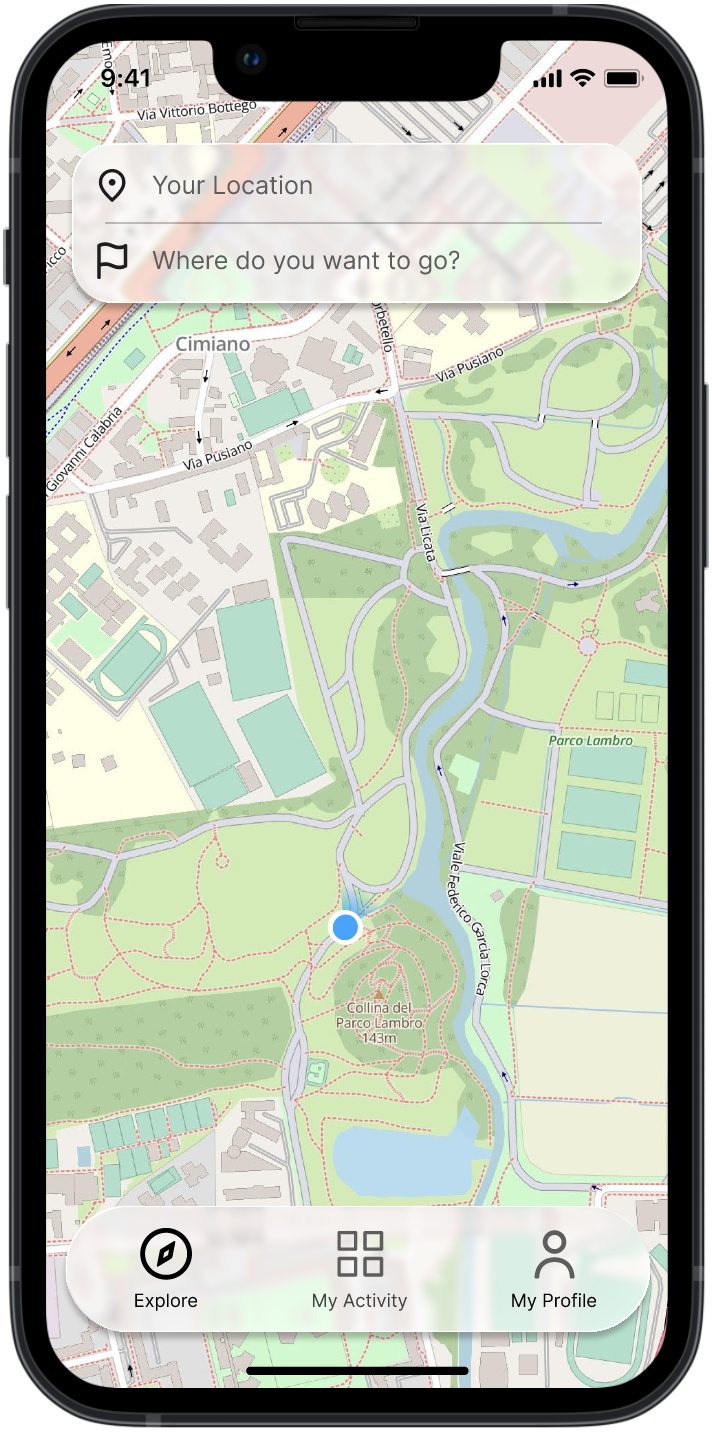
\includegraphics[width=\linewidth]{figures/mockup/search_path.png}
        \caption{Path Search Input}
        \label{fig:search_path_input}
    \end{subfigure}
    \hfill
    \begin{subfigure}{0.48\linewidth}
        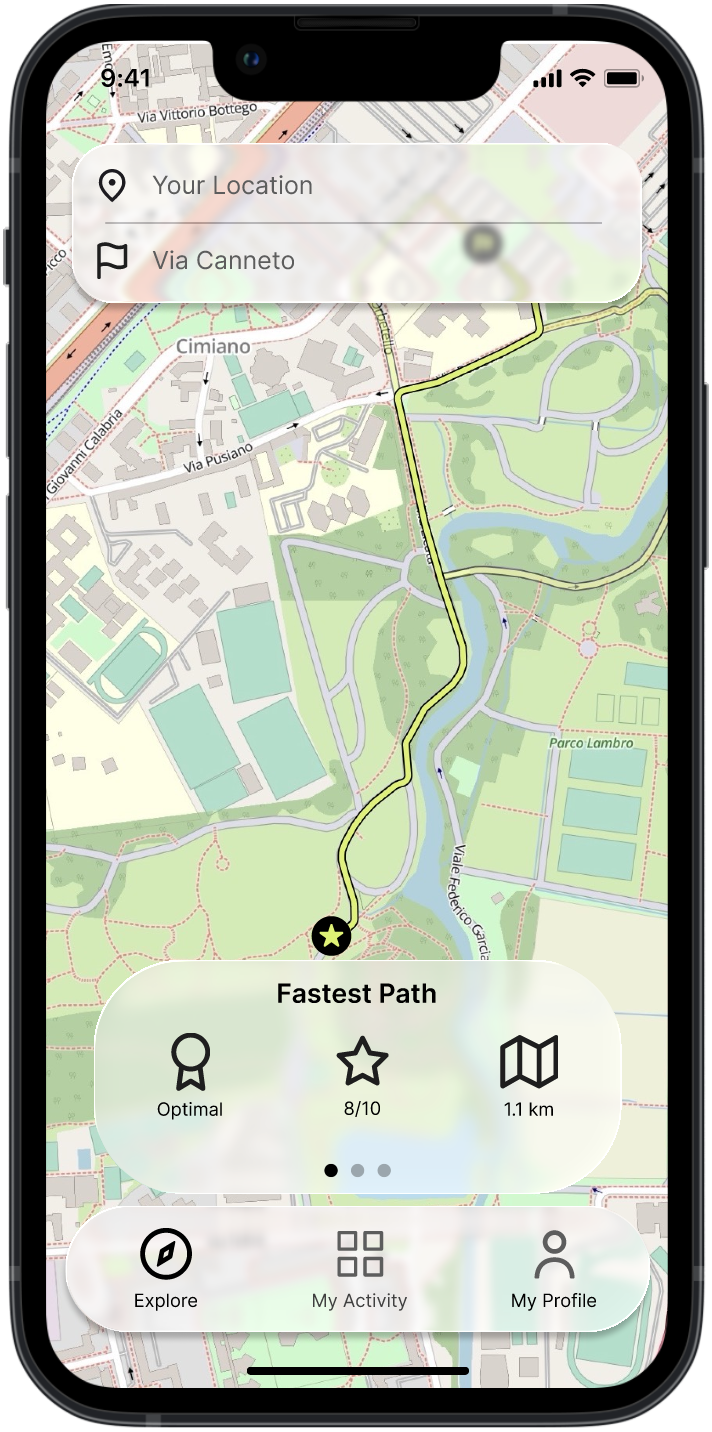
\includegraphics[width=\linewidth]{figures/mockup/search_path_result.png}
        \caption{Path Search Results}
        \label{fig:search_path_result}
    \end{subfigure}
    \caption{Path Search Screens}
    \label{fig:search_screen}
\end{minipage}

\subsubsection*{Recording}
\begin{minipage}[t]{0.45\textwidth}
    \setlength{\parindent}{7mm}
    \setlength{\parskip}{2mm}
    \vspace{0pt}
    \noindent
    The tracking functionality is managed through a sequence of interfaces designed to balance ease of use during physical activity with data accuracy during the final review.
    
    The \textbf{Active Recording Interface} is optimized for minimal distraction while moving. It features high-contrast typography and large touch targets to display real-time telemetry such as current speed, distance, and duration. A key visual element in this screen is the \emph{Auto-Pause indicator}, which provides immediate feedback when the System detects a stop or non-cycling movement (\eg, walking), ensuring the User is aware of the recording state. To prevent accidental interruptions during the ride, the stop command requires a deliberate interaction (\eg, a \emph{slide-to-confirm} gesture) rather than a simple tap.

    Upon concluding the session, the User transitions to the \textbf{Post-Ride Validation} screen. This interface is critical for the logic defined in the requirements. Before permanently saving the Trip and the associated Path, the User is presented with a summary of the collected data and is required to perform three validation tasks:
    \begin{enumerate}[noitemsep]
        \item \textbf{Obstacle Review:} A list of anomalies automatically detected by the sensors (\eg, potholes) is displayed for confirmation or rejection, filtering out false positives. The User can also add undetected obstacles manually.
        \item \textbf{Path Rating:} A control to assign a qualitative status to the Path and to some specific traversed segments.
        \item \textbf{Visibility:} Two buttons allowing the User to decide whether to keep the track \emph{Private} or publish it as \emph{Public} to contribute to the global map.
    \end{enumerate}
\end{minipage}
\hfill
\begin{minipage}[t]{0.5\textwidth}
    \vspace{0pt}
    \captionsetup{type=figure}
    \begin{subfigure}{0.48\linewidth}
        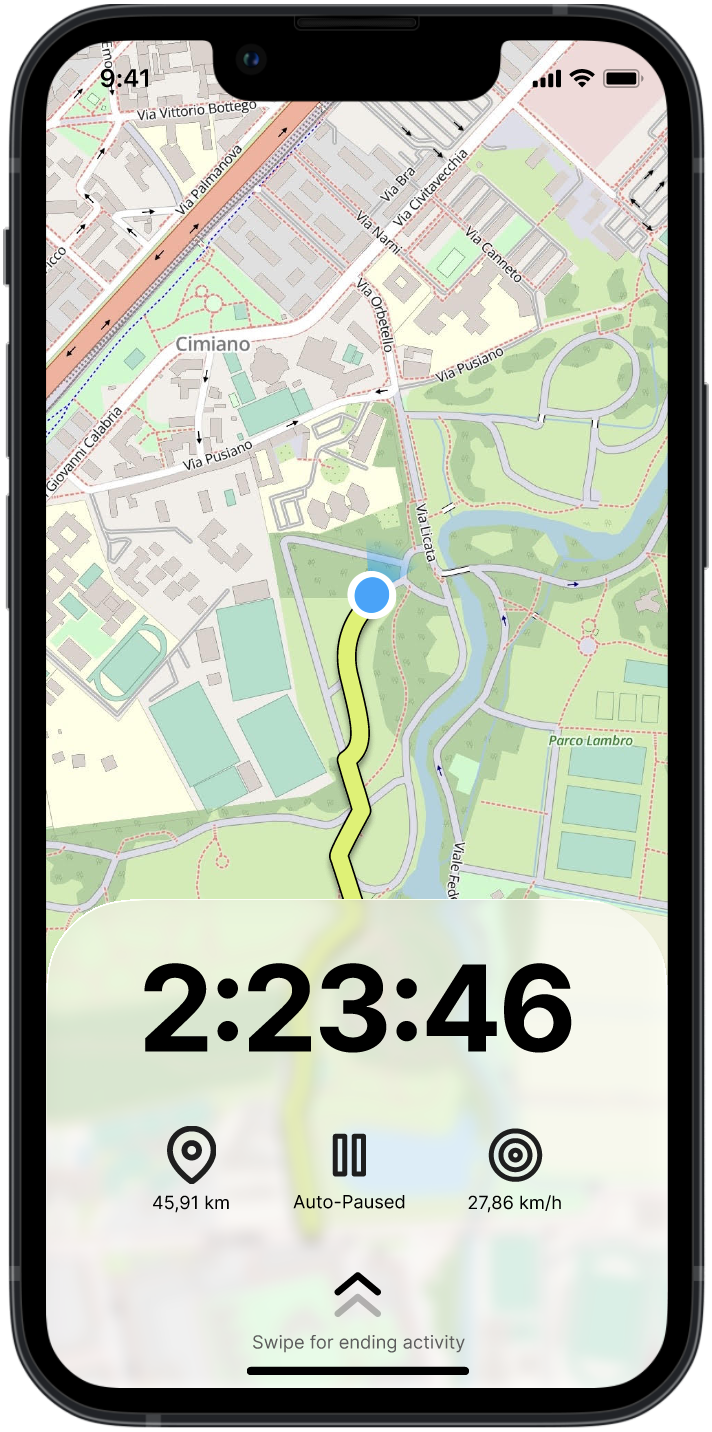
\includegraphics[width=\linewidth]{figures/mockup/during_a_trip.png}
        \caption{Compact View}
        \label{fig:during_a_trip}
    \end{subfigure}
    \hfill
    \begin{subfigure}{0.48\linewidth}
        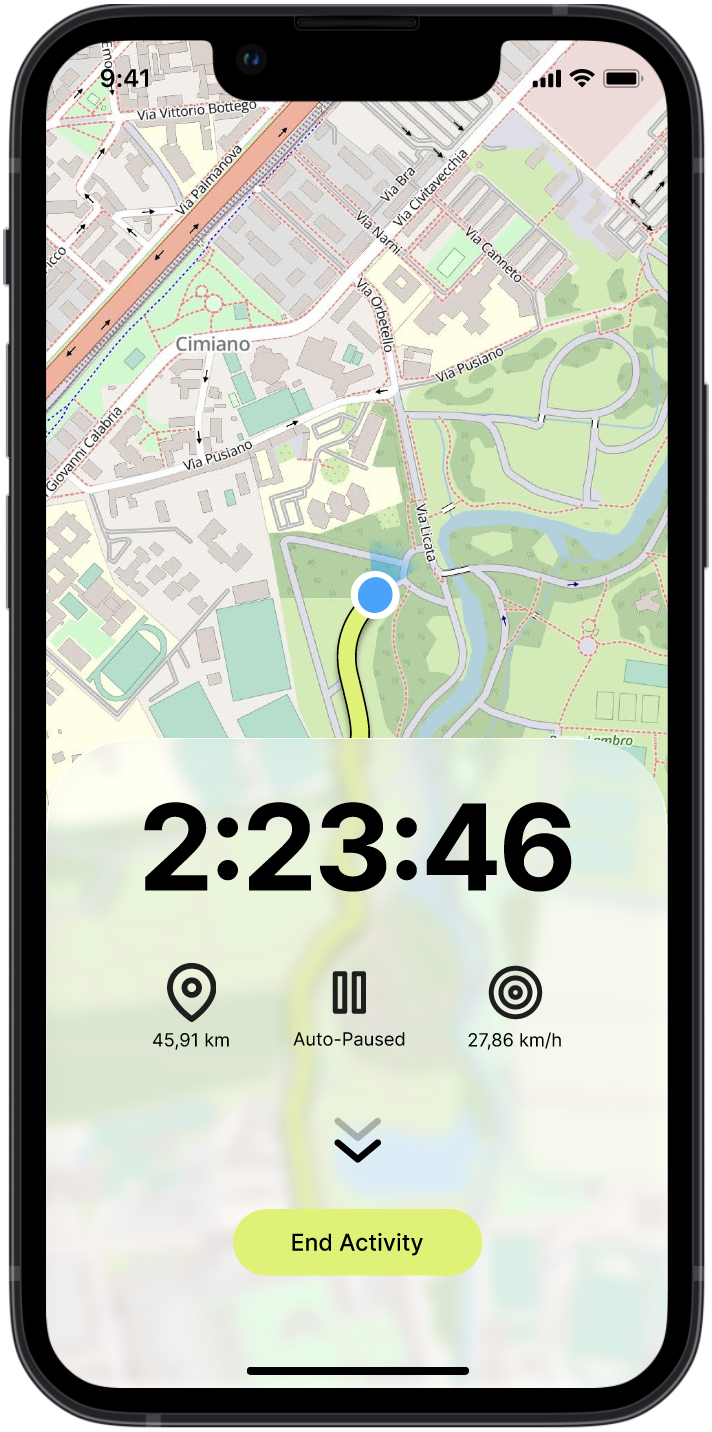
\includegraphics[width=\linewidth]{figures/mockup/ending_a_trip.png}
        \caption{Ending Confirmation}
        \label{fig:ending_a_trip}
    \end{subfigure}
    \begin{subfigure}{0.48\linewidth}
        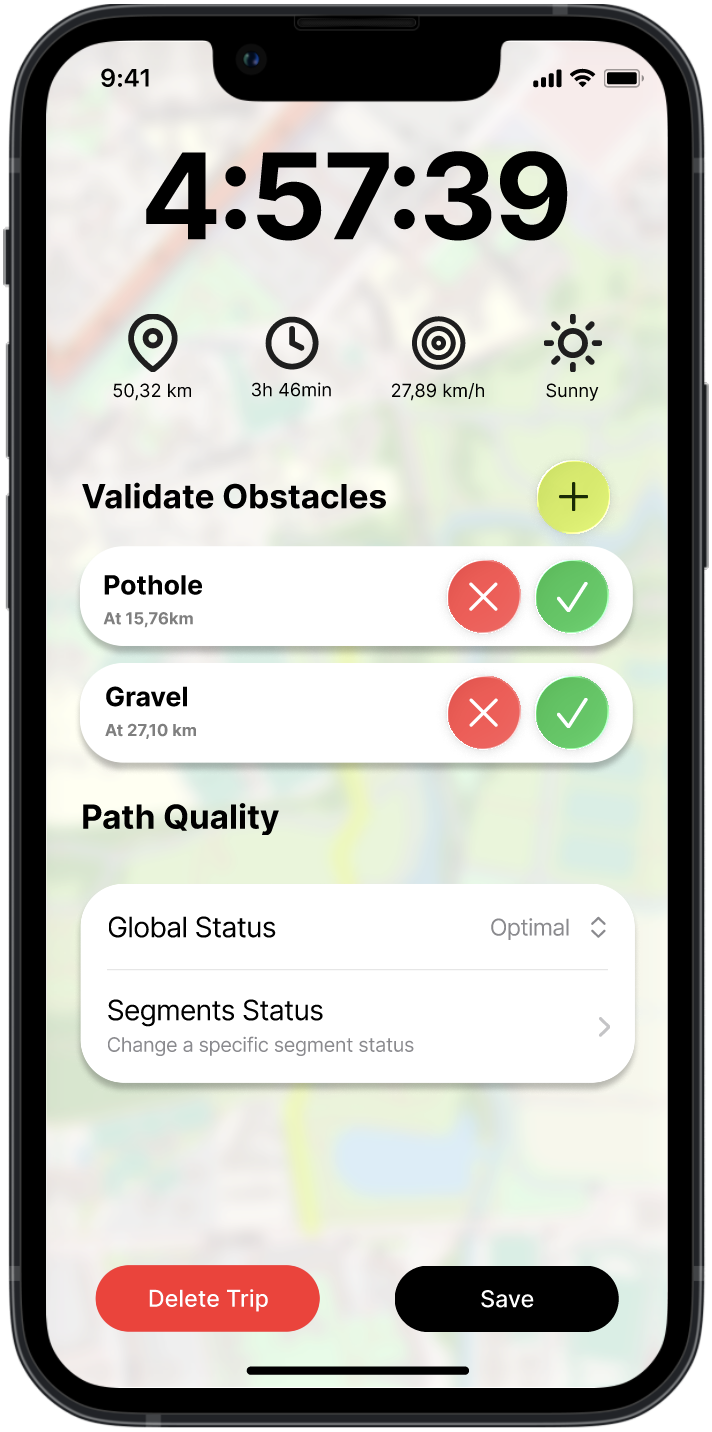
\includegraphics[width=\linewidth]{figures/mockup/validation.png}
        \caption{Trip Validation}
        \label{fig:validation}
    \end{subfigure}
    \hfill
    \begin{subfigure}{0.48\linewidth}
        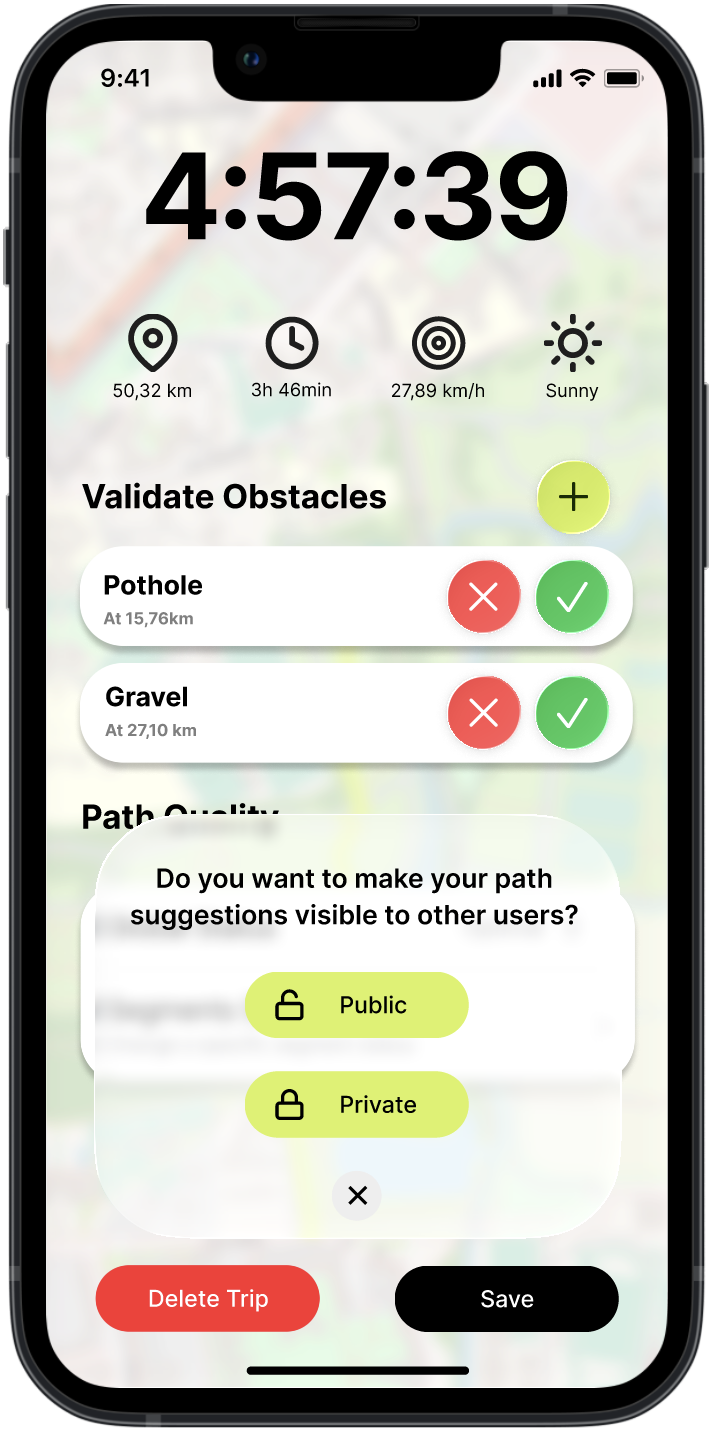
\includegraphics[width=\linewidth]{figures/mockup/validation_confirm.png}
        \caption{Path Visibility}
        \label{fig:validation_confirm}
    \end{subfigure}
    \caption{Mockups of Recording Screen}
    \label{fig:recording_screen}
\end{minipage}
\newpage
\subsection{Profile}

\begin{minipage}[t]{0.65\textwidth}
    \setlength{\parindent}{7mm}
    \setlength{\parskip}{2mm}
    \vspace{0pt}
    \noindent
    The Profile Section serves as the central hub for managing the User's identity and application preferences. For a \textbf{Registered User}, this interface acts as a personal dashboard displaying the account details defined in the domain model, such as name and surname.

    Beyond simple data visualization, the screen allows access to the \textbf{App Settings} submenu. Here, Users can configure technical parameters and manage privacy controls, including permissions for background sensor usage. In strict compliance with GDPR requirements, this section houses critical data management features, granting Users the ability to export their personal data or request the permanent deletion of their account and associated logs.

    The interface dynamically adapts its content based on the current session state. While registered Users are presented with a \textbf{Logout} option to securely terminate their session, \textbf{Guest Users} accessing this section view a restricted interface. Instead of personal details, they are presented with prompts to \textbf{Log In} or \textbf{Sign Up}, encouraging the transition from a transient anonymous session to a persistent account to unlock full platform capabilities. 
\end{minipage}
\hfill
\begin{minipage}[t]{0.30\textwidth}
    \vspace{0pt}
    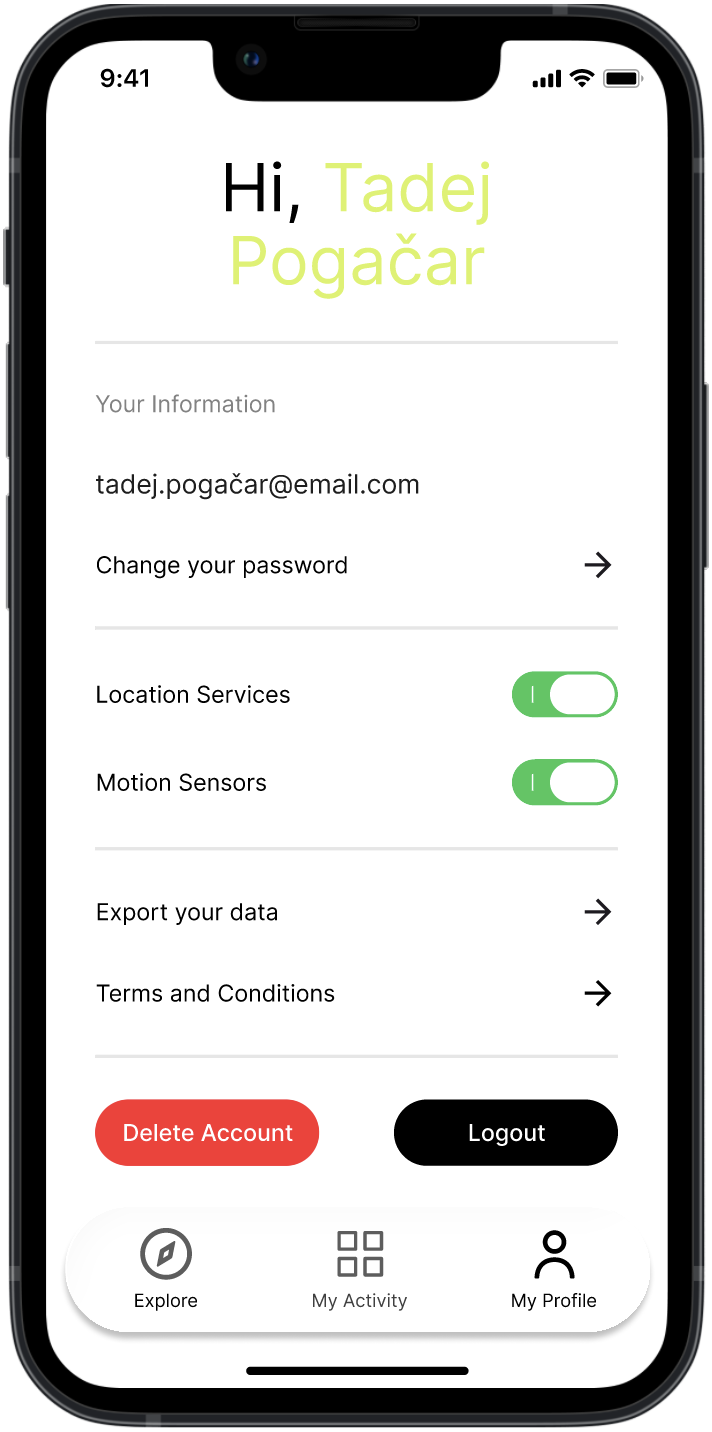
\includegraphics[width=\linewidth]{figures/mockup/profile_selection.png}
    \captionof{figure}{Profile Screen}
    \label{fig:profile_screen}
\end{minipage}

\subsection{My Activity}
\begin{minipage}[t]{0.65\textwidth}
    \setlength{\parindent}{7mm}
    \setlength{\parskip}{2mm}
    \vspace{0pt}
    \noindent
    The \textbf{My Activity} section acts as the comprehensive logbook for the Registered User, consolidating all historical data generated within the platform. Accessible directly from the main bottom navigation bar, this screen serves as the entry point for managing personal content.

    The interface is designed around a clear separation of concerns, subdividing the screen into two sections to allow Users to have a glance at their activity:
    \begin{itemize}[noitemsep]
        \item \textbf{Trips:} For accessing the chronological history of recorded performances.
        \item \textbf{Paths:} For managing the library of saved geographical Paths.
    \end{itemize}

    This layout ensures that Users can rapidly switch between reviewing their athletic performance and managing their map contributions without losing navigation context. By default, the screen opens on the most recent activity list, providing immediate access to the latest data. 
\end{minipage}
\hfill
\begin{minipage}[t]{0.3\textwidth}
    \vspace{0pt}
    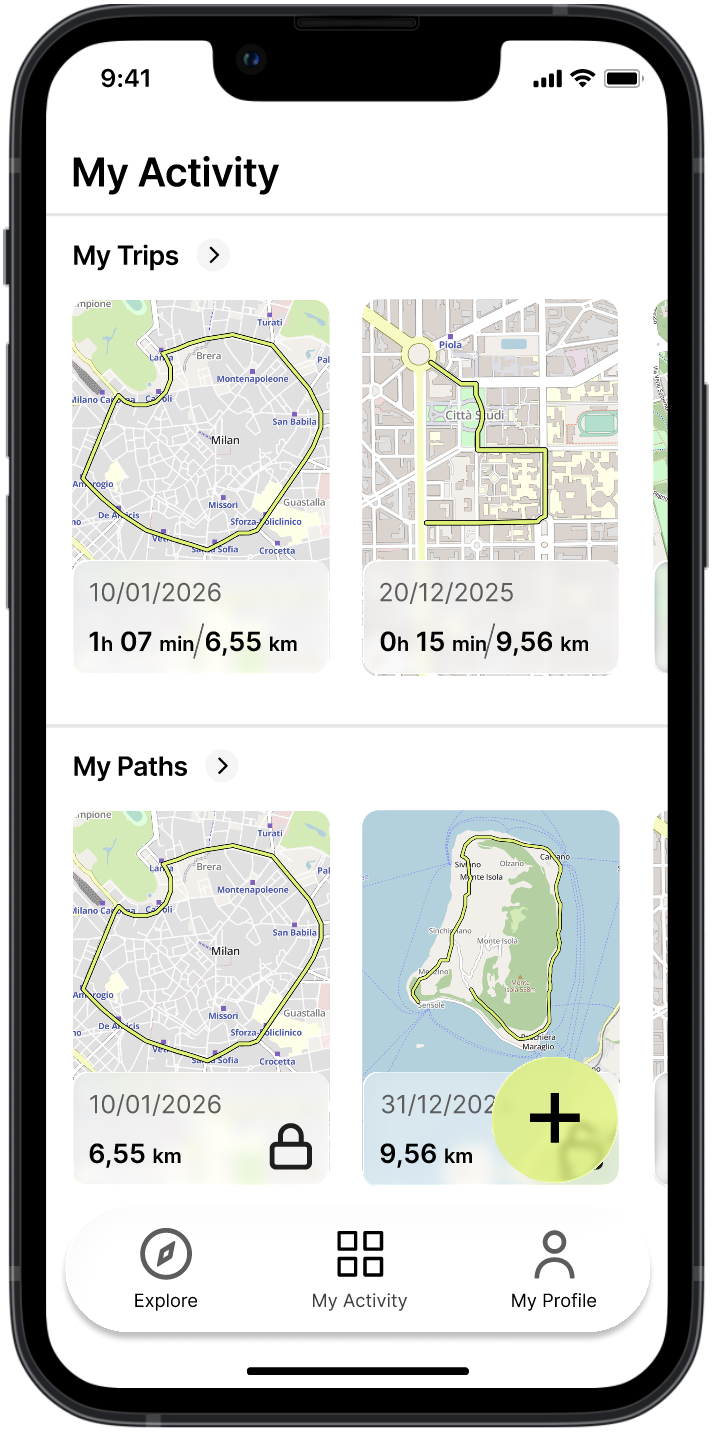
\includegraphics[width=\linewidth]{figures/mockup/my_activity.png}
    \captionof{figure}{My Activity Screen}
    \label{fig:my_activity_screen}
\end{minipage}

\subsubsection*{Trip Details}
\begin{minipage}[t]{0.45\textwidth}
    \setlength{\parindent}{7mm}
    \setlength{\parskip}{2mm}
    \vspace{0pt}
    \noindent
    Upon selecting a specific entry from the history list, the User is presented with the \textbf{Trip Detail} view. This interface offers a comprehensive post-ride analysis, visualizing the recorded track overlaid on the interactive map to allow Users to review the exact route taken.

    Below the geospatial representation, a dedicated dashboard displays the aggregated performance metrics captured during the session, including total distance, duration, average speed, and elevation gain. To provide a complete context for the athletic activity, the screen also presents the meteorological data (\eg, temperature and weather condition) retrieved from external services for that specific time and location. From this interface, the User retains full control over their data, with the specific option to permanently delete the recording from the System if deemed unnecessary.
\end{minipage}
\hfill
\begin{minipage}[t]{0.5\textwidth}
    \vspace{0pt}
    \captionsetup{type=figure}
    \begin{subfigure}{0.48\linewidth}
        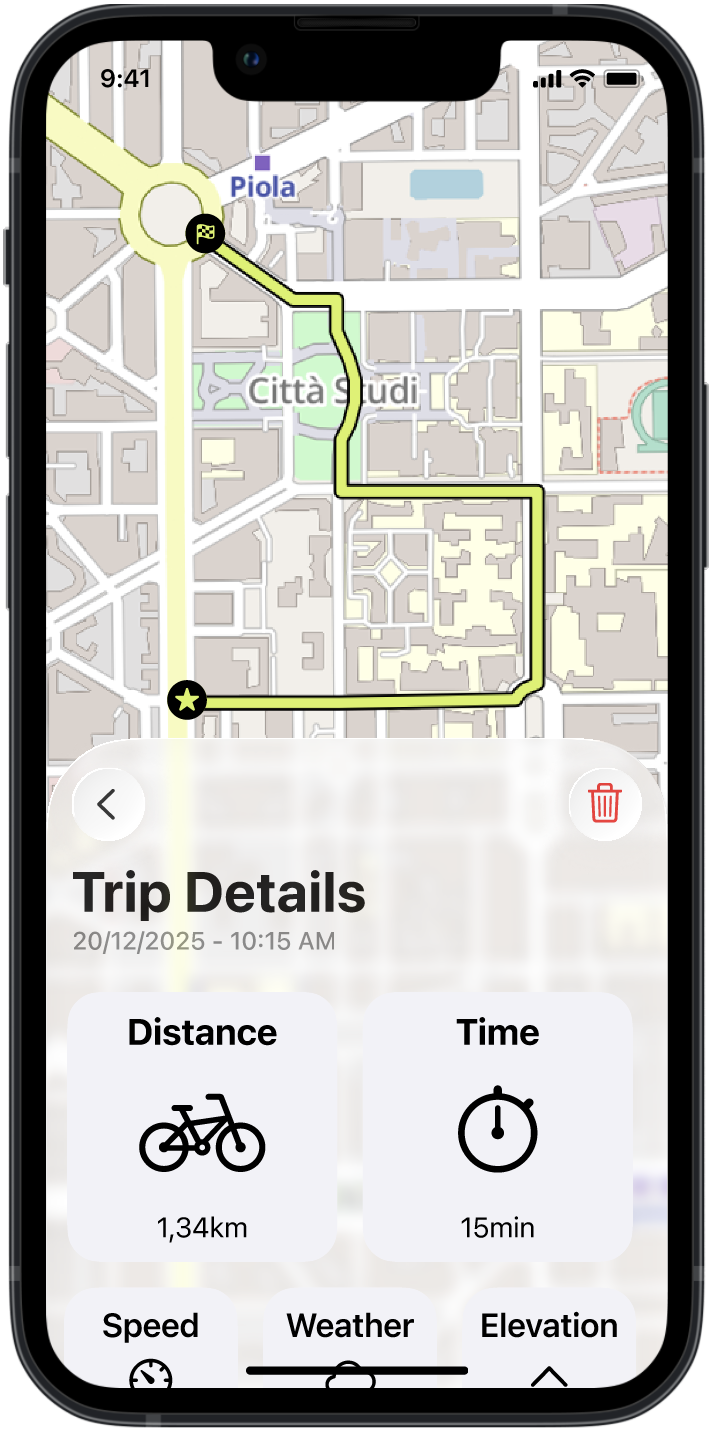
\includegraphics[width=\linewidth]{figures/mockup/trip_details.png}
        \caption{Compact View}
        \label{fig:trip_details}
    \end{subfigure}
    \hfill
    \begin{subfigure}{0.48\linewidth}
        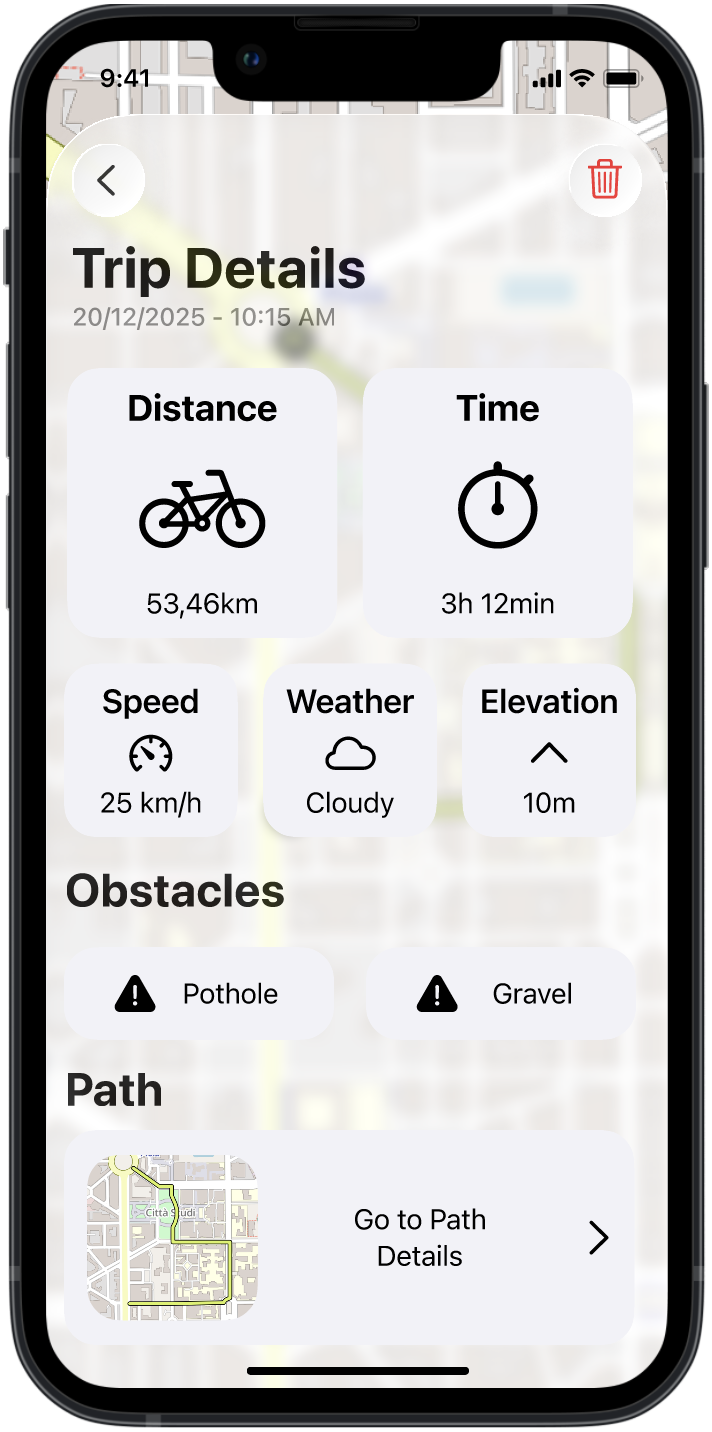
\includegraphics[width=\linewidth]{figures/mockup/trip_details_expanded.png}
        \caption{Expanded View}
        \label{fig:trip_details_expanded}
    \end{subfigure}
    \caption{Trip Details Screens}
\end{minipage}

\subsubsection*{Path Details}
\begin{minipage}[t]{0.65\textwidth}
    \setlength{\parindent}{7mm}
    \setlength{\parskip}{2mm}
    \vspace{0pt}
    \noindent
    Accessing an item from the Path Library opens the \textbf{Path Details} view, which focuses on the static geographical definition of the route. Unlike the Trip view, this interface highlights the qualitative attributes of the road network. The Path is rendered on the map, colour-coded according to its \textbf{Aggregated Status}, and accompanied by its calculated \emph{Reliability Score}.
    
    A central control in this interface is the \textbf{Visibility Button}. This feature empowers the User to manage the lifecycle of the data: they can choose to keep the Path \emph{Private} for personal use or switch it to \emph{Public}. Publishing the Path triggers the System's data aggregation algorithms, merging the User's local ratings with the global map to assist the entire community. Finally, the interface provides a specific option to delete the Path entity, ensuring the User retains full ownership of their content.
\end{minipage}
\hfill
\begin{minipage}[t]{0.30\textwidth}
    \vspace{0pt}
    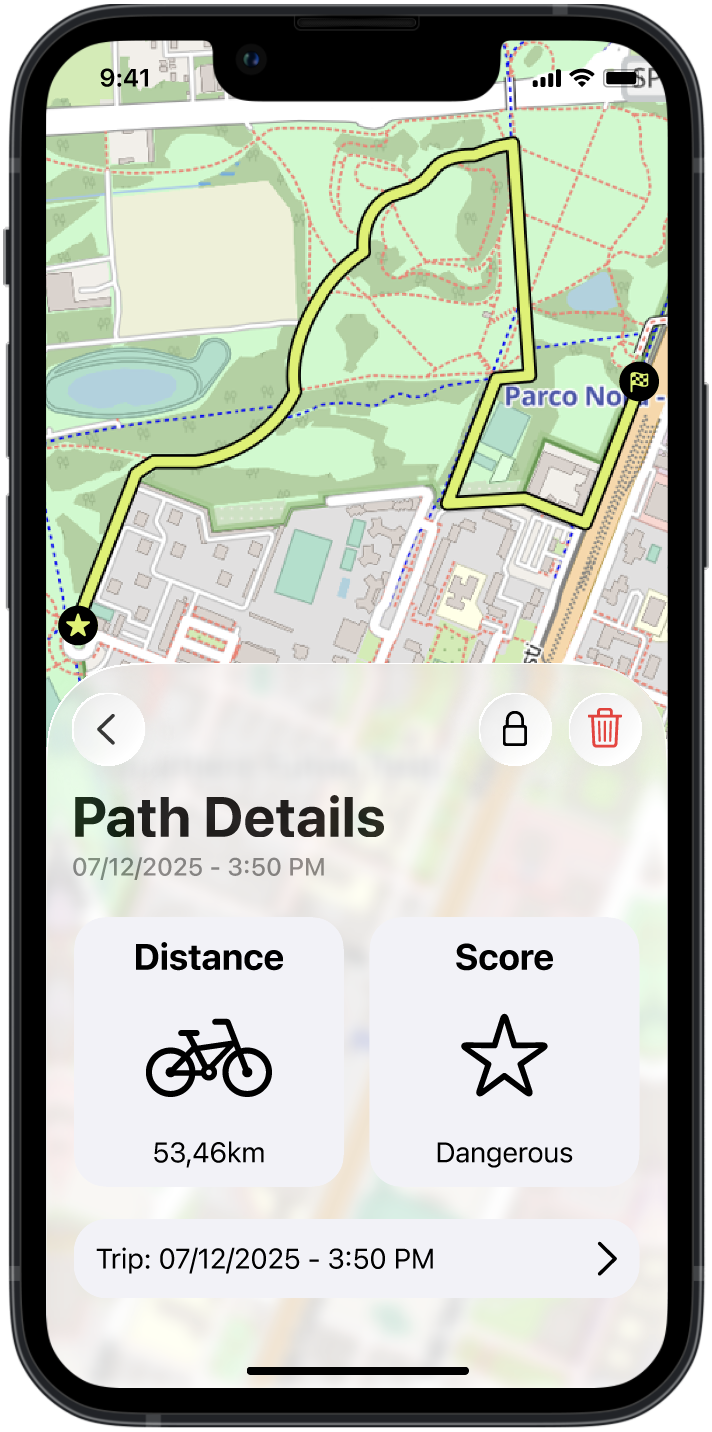
\includegraphics[width=\linewidth]{figures/mockup/path_details.png}
    \captionof{figure}{Path Details Screen}
    \label{fig:Path_details_screen}
\end{minipage}

\subsubsection*{Manual Path Creation}
\begin{minipage}[t]{0.45\textwidth}
    \setlength{\parindent}{7mm}
    \setlength{\parskip}{2mm}
    \vspace{0pt}
    \noindent
    The \textbf{Manual Path Creation} interface provides a dedicated toolset for Registered Users to contribute to the map inventory without the need for real-time tracking. This feature is particularly designed for expert Users who wish to map known trails or plan future routes from the comfort of their home.

    The workflow consists of two main stages. First, the User interacts with the \textbf{Track Editor}, selecting a sequence of waypoints on the map. The System automatically snaps these points to the underlying road network to reconstruct a valid, continuous geometry. 

    Once the route is defined, the interface transitions to the \textbf{Details Configuration} form. Here, the User assigns a global status to the Path to warn future cyclists. Advanced controls allow for granular overrides, enabling the User to mark specific segments with a different status if conditions vary along the route. Finally, the User sets the initial visibility permissions before saving the new entry to the database.
\end{minipage}
\hfill
\begin{minipage}[t]{0.5\textwidth}
    \vspace{0pt}
    \captionsetup{type=figure}
    \begin{subfigure}{0.48\linewidth}
        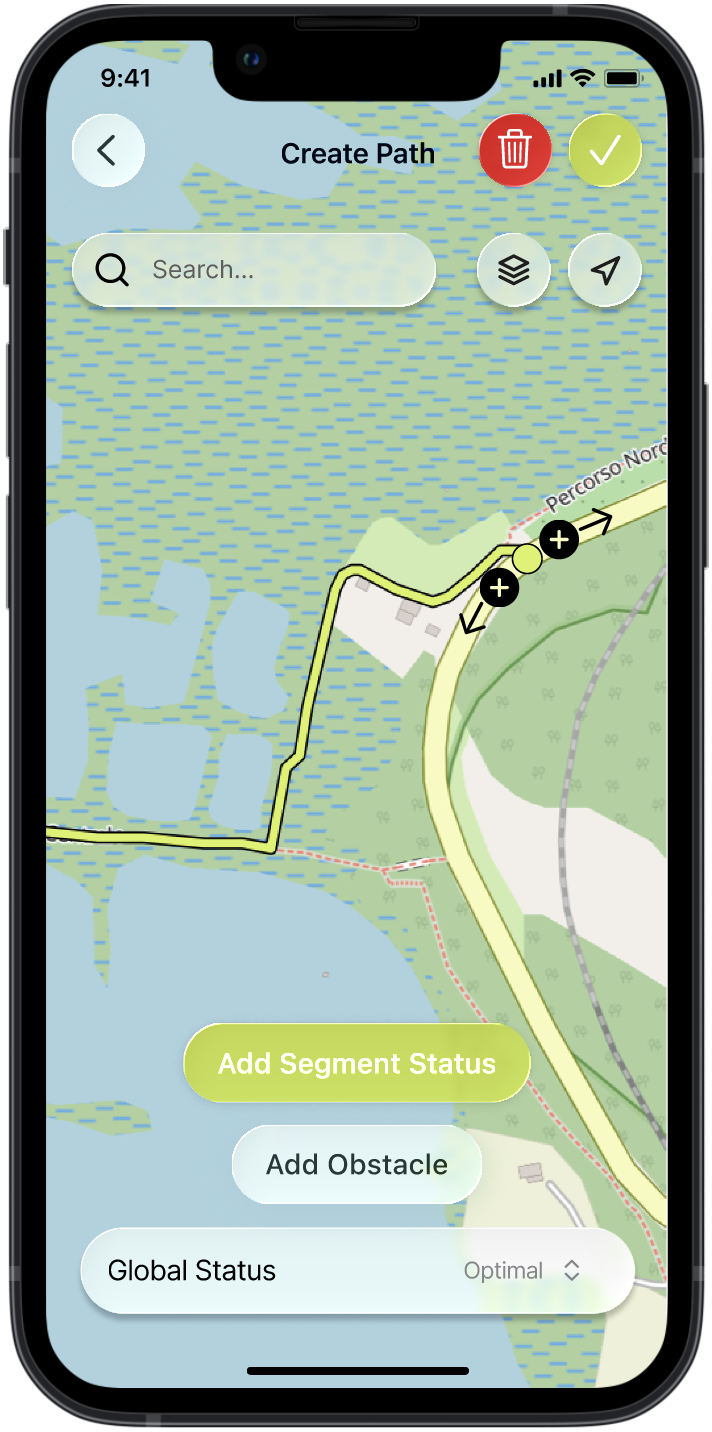
\includegraphics[width=\linewidth]{figures/mockup/create_path.png}
        \caption{Create a Path}
        \label{fig:create_path}
    \end{subfigure}
    \hfill
    \begin{subfigure}{0.48\linewidth}
        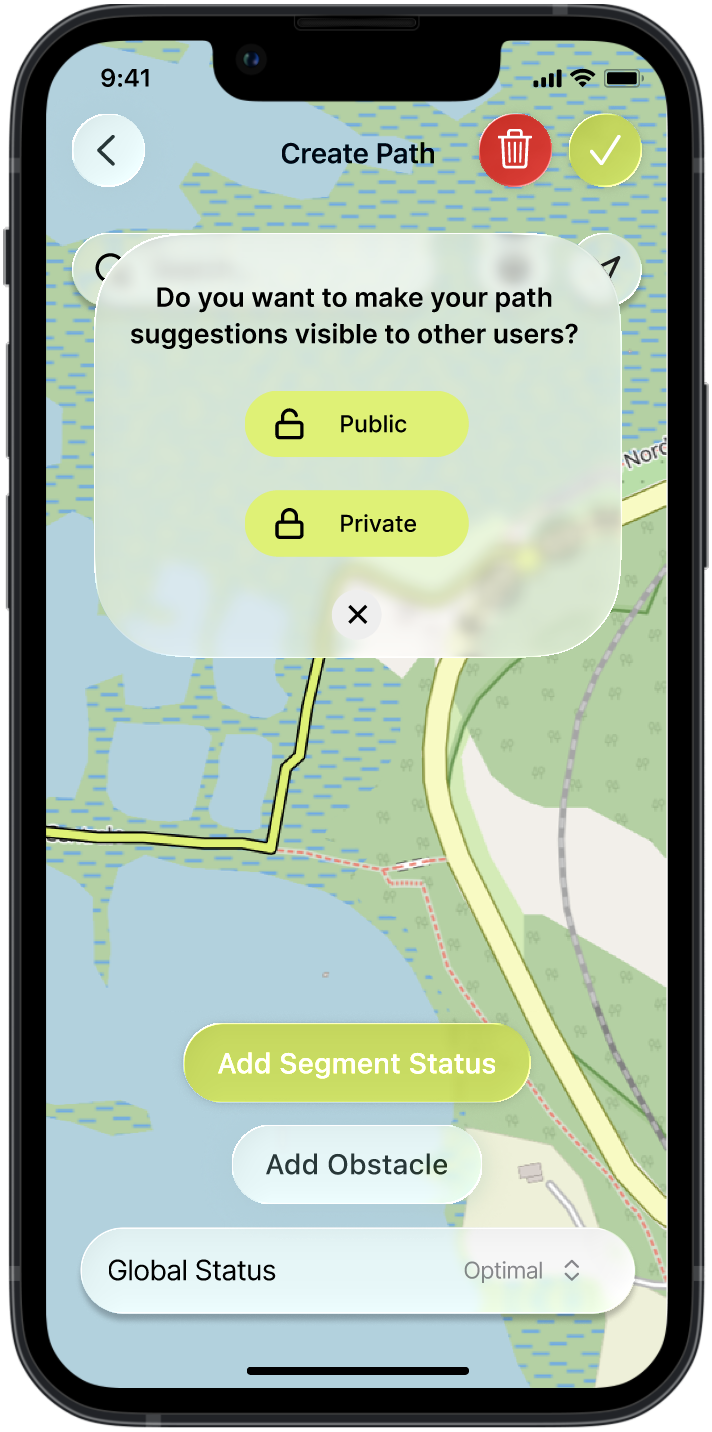
\includegraphics[width=\linewidth]{figures/mockup/create_path_confirm.png}
        \caption{Confirm a Path}
        \label{fig:create_path_confirm}
    \end{subfigure}
    \caption{Path Creation Screens}
\end{minipage}